\section{Examples for the Preceding Chapters (21K,22P)}
For clarification of the previous points, we will use examples, taking first a distinguished nativity:

% -- Chart 1 -------------------------------------------------
\subsection*{\textit{[Chart 1 Illustrious and Distinguished]}}
\addcontentsline{toc}{subsection}{\textit{[Chart 1 [GH L50] Illustrious and Distinguished]}}

\Sun\xspace in \Scorpio, \Moon\xspace in \Cancer, \Saturn\xspace in \Aquarius, \Jupiter\xspace in \Sagittarius, \Mars\xspace in \Scorpio, \Venus\xspace in \Libra, \Mercury\xspace in \Scorpio, Ascendant in \Libra
\footnote{\textit{Greek Horoscopes} dates the chart to approximately October 25, 50 A.D. (p.81)}. 

\clearpage
\begin{wrapfigure}[14]{R}{7cm}
\centering
\vspace{-20pt}
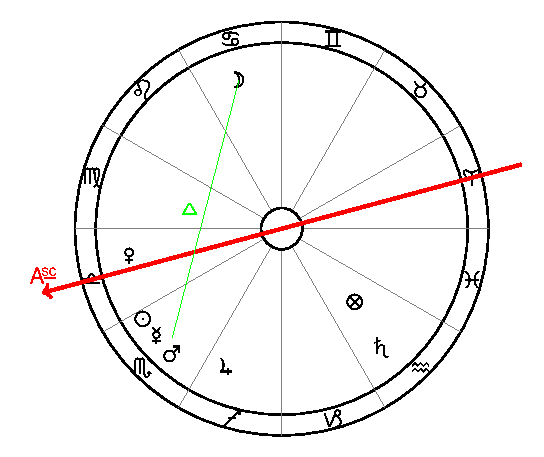
\includegraphics[width=.68\textwidth]{charts/2_21_1}
\caption{Chart 1 [II.22.1, GH L50]}
\label{fig:chart01}
\end{wrapfigure}

Since the birth was at night, I investigate the \Moon: this
happens to be in \Cancer, \Trine\xspace with \Mars. We find \Mars\xspace rising just after the Ascendant and in its own
house $<$\Scorpio$>$, triangle $<$\Scorpio\xspace\Pisces\xspace \Cancer$>$, and sect $<$nocturnal$>$\footnote{Must be referring to the chart sect as \Mars\xspace is placed below the horizon in the diurnal hemisphere and so out of sect.}. Then we find \Venus\xspace sharing rulership with \Mars, being in the Ascendant and in its own house $<$\Libra$>$. Third, we find the \Moon\xspace at MC in its own house $<$\Cancer$>$. It is obvious that the nativity is distinguished, since the houserulers are configured so appropriately. Investigating the Lot of Fortune, I find it in \Aquarius; \Saturn\xspace is there, the ruler $<$of \Aquarius$>$ and in $<$the V Place of$>$ Good Fortune, in its own house $<$\Aquarius$>$ and \textbf{/80P/} triangle $<$\Aquarius\xspace \Libra\xspace \Gemini$>$. Likewise the 11th Place from the Lot of Fortune, i.e. the Place of Accomplishment, is $<$\Sagittarius$>$, and \Jupiter\xspace is there.

I also found the exaltation of the nativity: from the \Moon\xspace to \Taurus\xspace is eleven signs, and the same distance from the Ascendant in \Libra\xspace brings me to \Leo, in $<$the XI Place of$>$ [the] Good Daimon. The \Sun\xspace is the ruler of this and since it is found to be at MC with respect to the Lot of Fortune, it made the birth even more illustrious and distinguished.
\newpage
% -- Chart 2 -------------------------------------------------
\subsection*{\textit{[Chart 2 Rise from Mediocrity]}}
\addcontentsline{toc}{subsection}{\textit{[Chart 2 [GH L95] Rise from Mediocrity]}}

Another example: \Sun, \Mercury\xspace in \Taurus, \Moon\xspace in \Aries, \Saturn, \Mars, \Venus, Ascendant in \Cancer,
\Jupiter\xspace in \Capricorn, \Fortune\xspace and the exaltation of the nativity in \Gemini
\footnote{\textit{Greek Horoscopes} has this as L95,V,II with \Saturn\xspace in \Leo\xspace and \Jupiter\xspace in \Virgo. According to GH, ``no date in the first three centuries of our era corresponds to the data of the text according to which \Saturn, \Mars, and \Venus\xspace should be in \Cancer'' (p.98); moving \Saturn\xspace into \Leo\xspace makes the chart almost parallel to example Chart 9 and places the date at approximately May 19, 95 A.D.. The alternate placements are shown in \textcolor{red}{red}.}.

\clearpage
\begin{wrapfigure}[16]{R}{7cm}
\centering
\vspace{-20pt}
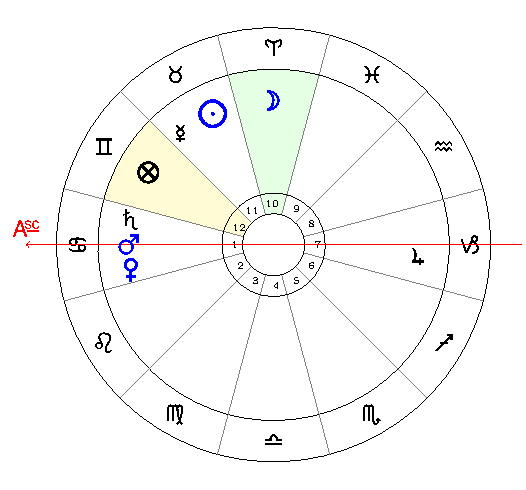
\includegraphics[width=.68\textwidth]{charts/2_21_2}
\caption{Chart 2 [II.21.2, GH L95,V,18]}
\label{fig:chart02}
\end{wrapfigure}

The native rose from mediocre origins to become a prefect and a governor. Since this was a day birth, I found the \Sun\xspace in the triangle of the \Moon\xspace $<$\Taurus\xspace \Virgo\xspace \Capricorn$>$ and its partners, \Venus\xspace and \Mars, at an angle $<$Ascendant$>$, the \textbf{/84K/} Lot of Fortune and the exaltation in \Gemini, just preceding an angle (hence the beginning of his life was humble), and its ruler $<$\Mercury$>$ in $<$the XI Place of$>$ [the] Good Daimon.
\newpage

% -- Chart 3 -------------------------------------------------
\subsection*{\textit{[Chart 3 Rise from Ordinary Means to Wealth]}}
\addcontentsline{toc}{subsection}{\textit{[Chart 3 [GH L85] Rise from Ordinary Means to Wealth]}}

Another example: \Sun, \Mars, \Venus, \Mercury\xspace in \Aquarius, \Moon, \Jupiter\xspace in \Scorpio, \Saturn\xspace in \Aries, Ascendant in \Leo
\footnote{\textit{Greek Horoscopes} dates the chart (L85) to February 5, 85 AD (p.93-4).}.

\clearpage
\begin{wrapfigure}[13]{R}{7cm}
\centering
\vspace{-20pt}
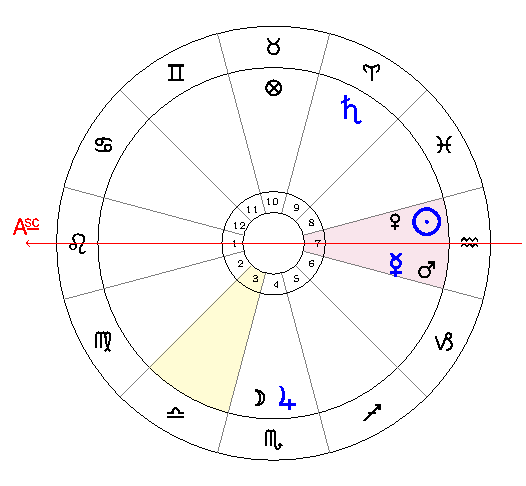
\includegraphics[width=0.68\textwidth]{charts/2_21_3}
\caption{Chart 3 [II.21.3, GH L85]}
\label{fig:chart03}
\end{wrapfigure}

This nativity also went from humble and ordinary fortune to the fortune of a prefect and a wealthy man. 

Since it was a day birth, we find the \Sun\xspace in the triangle of \Saturn\xspace $<$\Aquarius\xspace \Gemini\xspace \Libra$>$ with \Saturn\xspace just preceding an angle $<$MC$>$. Therefore his first years were ordinary. \Saturn’s partner, \Mercury, is at an angle $<$Descendant$>$. We find the Lot of Fortune in \Taurus, the exaltation in \Libra, and the ruler of these $<$\Venus$>$ is at MC relative to the Lot of Fortune and at an angle $<$Descendant$>$ otherwise $<$=relative to the Ascendant$>$.
\newpage
% -- Chart 4 -------------------------------------------------
\subsection*{\textit{[Chart 4 Rise through Violent Means]}}
\addcontentsline{toc}{subsection}{\textit{[Chart 4 [GH L83] Rise through Violent Means]}}

Another example: \Sun, \Mercury\xspace in \Taurus, \Moon\xspace in \Aquarius, \Saturn, \Venus\xspace in \Aries, \Jupiter\xspace in \Virgo, \Mars\xspace in \Pisces, Ascendant in \Leo
\footnote{\textit{Greek Horoscopes} dates the chart to approximately April 28, 83 AD (p.93). Valen also uses it as an example chart in Book II.36. A day birth.}

\clearpage
\begin{wrapfigure}[14]{R}{7cm}
\centering
\vspace{-20pt}
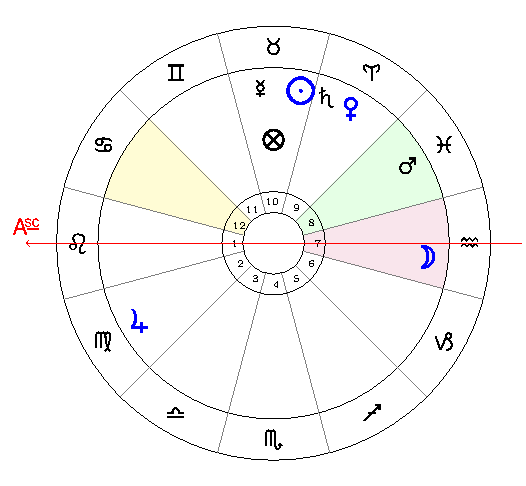
\includegraphics[width=.68\textwidth]{charts/2_21_4}
\caption{Chart 4 [II.21.4, GH L83]}
\label{fig:chart04}
\end{wrapfigure}

We find the \Sun\xspace in the triangle of \Venus\xspace and the \Moon\xspace $<$\Taurus\xspace \Virgo\xspace \Capricorn$>$ with \Venus\xspace preceding an angle $<$MC$>$. So the native’s life was at first burdened and lowly, but since the \Moon\xspace is at an angle $<$Descendant$>$, later he came into governmental and advantageous circumstances. Likewise the Lot of Fortune was found in \Taurus, the exaltation in \Cancer. The \Moon, the ruler of \Cancer, was found at MC relative to the Lot of Fortune; therefore the native came into great fortune and governorship. \Mars\xspace is found in the Place of Accomplishment, $<$which gave to him$>$ property from plunder, stealing, and violence, property which after his death was plundered most abominably.
\newpage
% -- Chart 5 -------------------------------------------------
\subsection*{\textit{[Chart 5 From Servitude to Power]}}
\addcontentsline{toc}{subsection}{\textit{[Chart 5 [GH L74] From Servitude to Power]}}

Another example: \Sun, \Mercury, \Saturn, \Jupiter\xspace in \Sagittarius, \Moon\xspace in \Cancer, \Mars\xspace in \Virgo,
\Venus, Ascendant in \Libra
\footnote{\textit{Greek Horoscopes} dates the chart (L74.XI) to approximately November 26, 74 AD. It is also used as an example in Book VII.36 where the MC is given as being in \Cancer. A night birth.}.

\clearpage
\begin{wrapfigure}[16]{R}{7cm}
\centering
\vspace{-20pt}
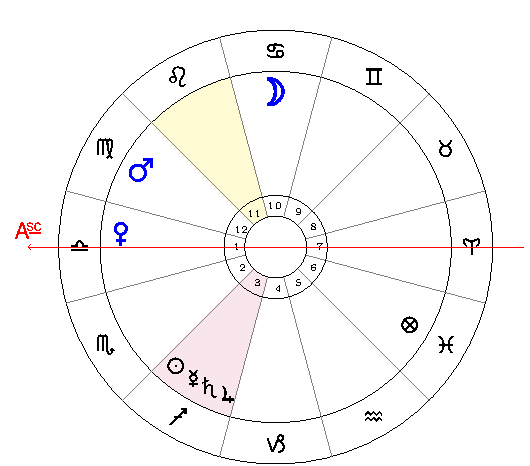
\includegraphics[width=0.68\textwidth]{charts/2_21_5}
\caption{Chart 5 [II.21.5, GH L74.XI]}
\label{fig:chart05}
\end{wrapfigure}

Since this was a night birth, \textbf{/81P/} we find the \Moon\xspace in the triangle of \Mars\xspace $<$\Cancer\xspace \Scorpio\xspace \Pisces$>$ with \Mars\xspace itself and the Lot of Fortune and its ruler $<$\Jupiter$>$ preceding angles.
Therefore he lived his first years humbly and in poverty; he experienced captivity and servitude and was involved in many dangers. But since the stars of the same sect happened to be in operative places, he came into friendships and associations and received positions of royal trust. Since the exaltation of the nativity was found in \Leo, and its ruler, the \Sun, was at MC relative to the Lot of Fortune, he was thought worthy of the governorship and a position of power.
\newpage

% -- Chart 6 -------------------------------------------------
\subsection*{\textit{[Chart 6 Rise to High Priesthood]}}
\addcontentsline{toc}{subsection}{\textit{[Chart 6 [GH L72] Rise to High Priesthood]}}

Another example: \Sun, \Mercury\xspace in \Capricorn, \Moon, \Venus\xspace in \Sagittarius, \Saturn\xspace in \Scorpio,
\Jupiter\xspace in \Libra, \Mars\xspace in \Aquarius, \Fortune \xspace in \Aries, Ascendant in \Taurus
\footnote{\textit{Greek Horoscopes} dates the chart (L72) to approximately January 6, 72 AD (p.85).}.

\clearpage
\begin{wrapfigure}{R}{7cm}
\centering
\vspace{-20pt}
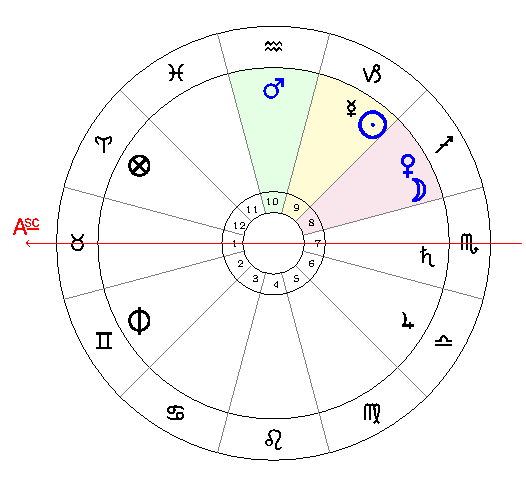
\includegraphics[width=0.68\textwidth]{charts/2_21_6}
\caption{Chart 6 [II.21.6, GH L72]}
\label{fig:chart06}
\end{wrapfigure}

This nativity too was at first irregular and mediocre, but later he rose and gained chaplets and a high priesthood. 

The rulers of the triangle $<$of the Lot of Fortune: \Taurus\xspace \Virgo\xspace \Capricorn$>$
\footnote{Fortune is in \Aries; the \Taurus-\Virgo-\Capricorn\xspace triplicity is the tricplicity of the sect light, the \Sun\xspace in \Capricorn\xspace.}  were found to be following an angle $<$Descendant$>$, and the third ruler $<$\Mars$>$ of the triangle and the ruler of the Lot were at MC. Likewise the ruler $<$\Sun$>$ of the exaltation of the nativity $<$\Leo$>$ was at MC relative to the Lot of Fortune, as was the ruler $<$\Mercury$>$ of Daimon $<$\Gemini$>$

\newpage
% -- Chart 7 -------------------------------------------------
\subsection*{\textit{[Chart 7 Rise to High Priesthood]}}
\addcontentsline{toc}{subsection}{\textit{[Chart 7 [GH L82] Rise to High Priesthood]}}

Another example: \Sun, \Mercury\xspace in \Cancer, \Moon\xspace in \Taurus, \Saturn\xspace in \Pisces, \Jupiter, \Mars\xspace in \Leo, \Venus\xspace in \Virgo, Ascendant in \Libra \footnote{\textit{Greek Horoscopes} dates the chart (L82) to approximately July 9, 82 AD (p.92)}.

\clearpage
\begin{wrapfigure}[16]{R}{7cm}
\centering
\vspace{-20pt}
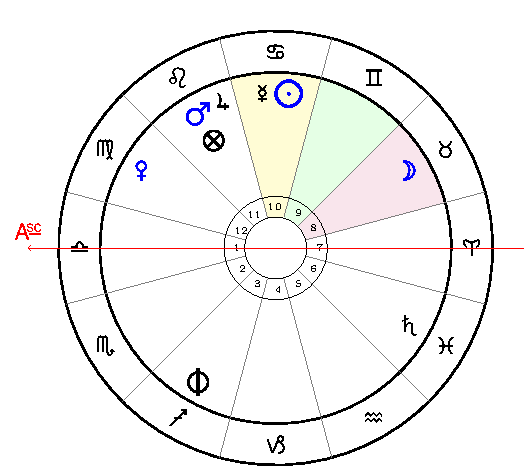
\includegraphics[width=0.68\textwidth]{charts/2_21_7}
\caption{Chart 7 [II.21.7, GH L82]}
\label{fig:chart07}
\end{wrapfigure}

This nativity too was illustrious and distinguished. The native was entrusted with royal office and was thought worthy of a high priesthood. The ruler $<$\Mars$>$ of the triangle
$<$\Cancer\xspace \Scorpio\xspace \Pisces$>$ was found with the ruler of Daimon $<$\Jupiter$>$ in $<$the XI Place of$>$ Good Daimon and with the Lot of Fortune. The \Sun, at MC, was assigned the Lot. The ruler of the exaltation, the \Moon, was at MC relative to the Lot of Fortune. The Place of Accomplishment was irregular and unstable, sometimes being too full, at other times empty, for \Saturn\xspace and \Venus\xspace were in aspect to it $<$\Square$>$.

\newpage

% -- Chart 8 -------------------------------------------------
\subsection*{\textit{[Chart 8 Raised Livelihood]}}
\addcontentsline{toc}{subsection}{\textit{[Chart 8 [GH L97] Raised Livelihood]}}

Another example: \Sun, \Jupiter, \Mars, \Venus in \Scorpio, \Saturn\xspace in \Libra, \Moon\xspace in \Aries, \Mercury\xspace in \Sagittarius, Ascendant in \Leo
\footnote{\textit{Greek Horoscopes} dates the chart (L97,XI) to approximately November 6, 97 AD (p.99)}.

\clearpage
\begin{wrapfigure}[14]{R}{7cm}
\centering
\vspace{-20pt}
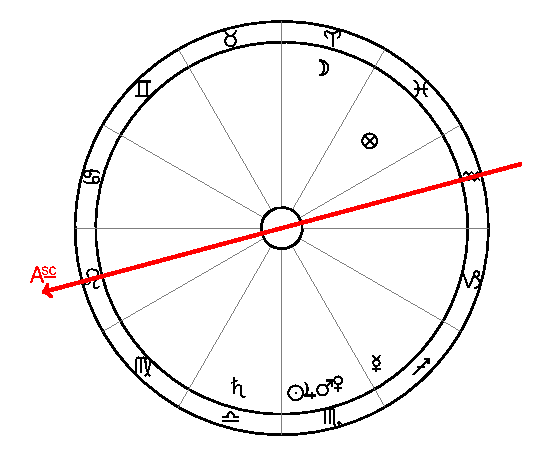
\includegraphics[width=0.68\textwidth]{charts/2_21_8}
\caption{Chart 8 [II.21.8, GH L97,XI]}
\label{fig:chart08}
\end{wrapfigure}

The ruler of the exaltation, \Mercury, was found in \Sagittarius, at MC relative to the Lot of Fortune\footnote{If \Sagittarius\xspace is the 10th from Fortune, the Lot must be in \Pisces.}, and it elevated the nativity with respect to livelihood. Likewise the rulers $<$\Sun, \Jupiter$>$ of the triangle $<$of the \Sun: \Aries-\Leo-\Sagittarius$>$ and of the Lot of Fortune\footnote{\Jupiter\xspace rules Fortune in \Pisces.} were found at IC. This made him miserly, unambitious, and niggardly.

\newpage
% -- Chart 9 -------------------------------------------------
\subsection*{\textit{[Chart 9 From Debt to Inheritance and Business Prosperity]}}
\addcontentsline{toc}{subsection}{\textit{[Chart 9 [GH L95] From Debt to Inheritance and Business Prosperity}}

Another example: \Sun, \Mercury\xspace in \Taurus, \Moon\xspace in \Aquarius, \Saturn\xspace in \Leo, \Mars, \Venus\xspace in \Cancer, \Jupiter\xspace in \Virgo, Ascendant in \Sagittarius
\footnote{\textit{Greek Horoscopes} dates the chart (L95,V) to approximately May 14, 95 AD (p.97)}.

\clearpage
\begin{wrapfigure}{R}{7cm}
\centering
\vspace{-20pt}
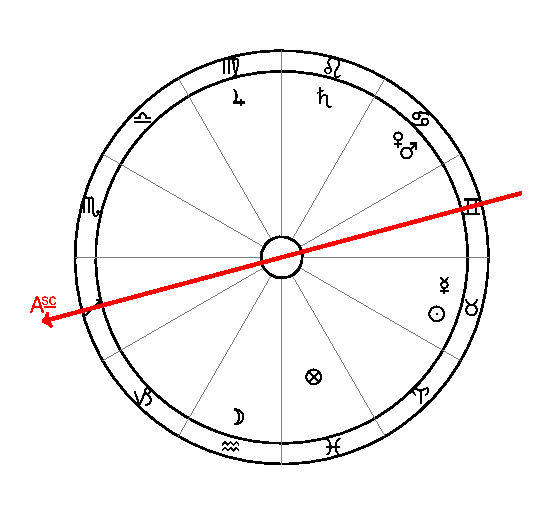
\includegraphics[width=0.68\textwidth]{charts/2_21_9}
\caption{Chart 9 [II.21.9, GH L95,V]}
\label{fig:chart09}
\end{wrapfigure}

Since this was a night birth, the rulers, \Saturn\xspace and \Mercury, of the triangle $<$\Gemini-\Libra-\Aquarius$>$ just preceded angles $<$MC Ascendant\footnote{Precedes the Descendant, not Ascendant.}$>$. \textbf{/82P/} Therefore he had many ups and downs in his early years and lived in debt, although the basis $<$of the nativity$>$ was good
with respect to parents. Later he got an inheritance and improved his means by profitable enterprises, and he became ambitious, dominant, and munificent. He was popular with the masses and a friend of kings \textbf{/86K/} and governors. He supplied temples and public works and gained perpetual remembrance. The Lot of Fortune and the exaltation were found in \Pisces, and its ruler, \Jupiter, was at MC.
\newpage
% -- Chart 10 -----------------------------------------------
\subsection*{\textit{[Chart 10 Born into Wealth]}}
\addcontentsline{toc}{subsection}{\textit{[Chart 10 [GH L65] Born into Wealth]}}

Another example: \Sun, \Mercury\xspace in \Scorpio, \Moon\xspace in \Aries, \Saturn\xspace in \Virgo, \Jupiter\xspace in \Pisces, \Mars\xspace in \Leo, \Venus, Ascendant in \Sagittarius
\footnote{\textit{Greek Horoscopes} dates the chart (L65,X) to approximately October 31, 65 AD (p.85) but claims the date is ``plausible...[but] a tentative solution'' as they feel ``some elements [as given in the text] must be wrong''}.

\clearpage
\begin{wrapfigure}[14]{R}{7cm}
\centering
\vspace{-20pt}
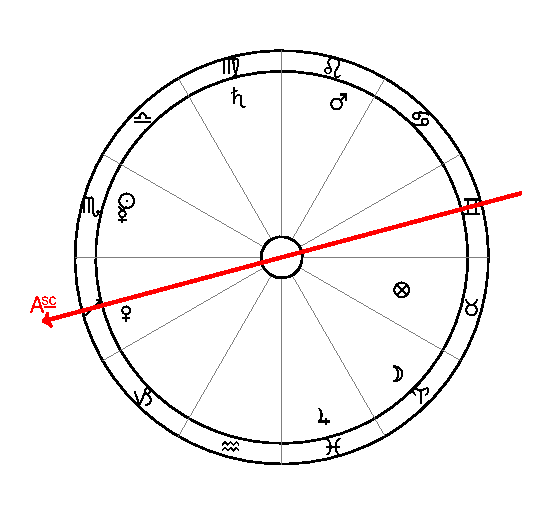
\includegraphics[width=0.68\textwidth]{charts/2_21_10}
\caption{Chart 10 [II.21.10, GH L65,X]}
\label{fig:chart10}
\end{wrapfigure}

Even when he was a child, the nativity inherited great property. The Place of Accomplishment was in \Pisces, with \Jupiter\xspace in its own house. \Venus, the co-ruler of the
triangle, the Lot of Fortune
\footnote{Calculated as Asc + (\Moon\xspace\xspace - \Sun) = \Sagittarius\xspace + (\Aries\xspace - \Virgo) = 240 + (360 - 150) = 30 or \Taurus.}
\clearpage

\newpage
% -- Chart 11 -----------------------------------------------
\subsection*{\textit{[Chart 11 Prosperity to Exile]}}
\addcontentsline{toc}{subsection}{\textit{[Chart 11 [GH L105] Prosperity to Exile]}}

Another example: \Sun, \Mercury\xspace in \Capricorn, \Moon, \Saturn\xspace in \Sagittarius, \Jupiter\xspace in \Cancer, \Mars\xspace in \Virgo, \Venus\xspace in \Aquarius, Ascendant in \Libra
\footnote{\textit{Greek Horoscopes} dates the chart (L65,X) to approximately January 1, 105 AD (p.103)}.

\clearpage
\begin{wrapfigure}[14]{R}{7cm}
\centering
\vspace{-20pt}
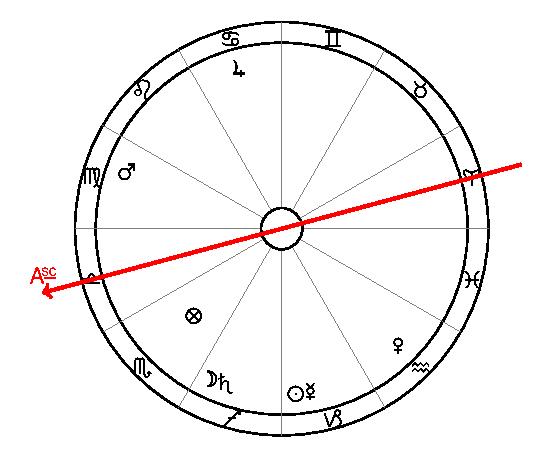
\includegraphics[width=0.68\textwidth]{charts/2_21_11}
\caption{Chart 11 [II.21.11, GH L105]}
\label{fig:chart11}
\end{wrapfigure}

The rulers $<$\Jupiter, \Sun$>$ of the triangle $<$of the \Sun$>$ were found at angles, but in opposition $<$MC IC$>$. Therefore the nativity, though well provided for and prosperous at first, was later found to be exiled and needy because of burning and plunder. The ruler of the Lot of Fortune, \Mars, was found in the Place of Accomplishment, but preceding an angle $<$Ascendant$>$ and in aspect with \Saturn $<$\Square$>$.

\newpage
% -- Chart 12 -----------------------------------------------
\subsection*{\textit{[Chart 12 Political Prestige to Vagabond]}}
\addcontentsline{toc}{subsection}{\textit{[Chart 12 [GH L61] Political Prestige to Vagabond]}}

Another example: \Sun, \Venus, Ascendant in \Taurus, \Moon\xspace in \Aquarius, \Saturn\xspace in \Cancer, \Jupiter\xspace in \Libra, \Mars, \Mercury\xspace in \Gemini
\footnote{\textit{Greek Horoscopes} dates the chart (L61,V) to approximately May 1, 61 AD (p.81)}.

\clearpage
\begin{wrapfigure}[14]{R}{7cm}
\centering
\vspace{-20pt}
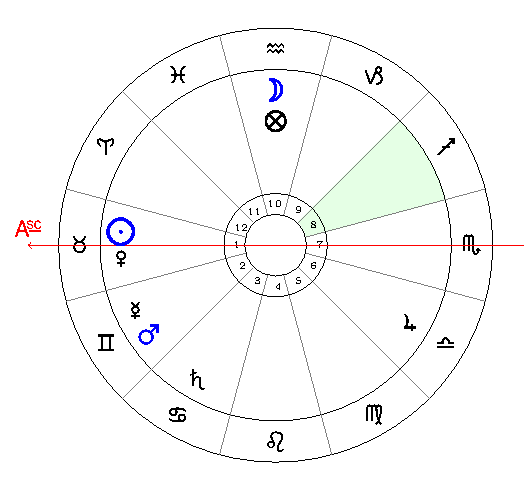
\includegraphics[width=0.68\textwidth]{charts/2_21_12}
\caption{Chart 12 [II.21.12, GH L61,V]}
\label{fig:chart12}
\end{wrapfigure}

In his first years, the native had great political prestige, affairs, and positions of trust. The rulers $<$\Venus\xspace \Moon$>$ of the triangle $<$\Taurus-\Virgo-\Capricorn$>$ happened to be at angles $<$Ascendant, MC$>$. Later his livelihood was ruined and he become a vagabond. \Mars\xspace and \Mercury\xspace were in opposition to the Place of Accomplishment and the rulers $<$\Saturn\xspace \Jupiter$>$ of the Lot\footnote{Lot of Fortune = Asc + (\Moon\xspace\xspace - \Sun) = 30 + (300 - 30) = 300, \Aquarius, ruled by \Saturn. The place of Accomplishment is in the 11th from the Fortune, here, \Sagittarius, ruled by \Jupiter.}
 and of the Place of Accomplishment preceded angles $<$IC Descendant$>$.
 
\newpage
% -- Chart 13 -----------------------------------------------
\subsection*{\textit{[Chart 13 From Slavery to Honors]}}
\addcontentsline{toc}{subsection}{\textit{[Chart 13 [GH L109] From Slavery to Honors]}}

Another example: \Sun, \Mercury\xspace in \Gemini,\Moon\xspace in \Capricorn, \Saturn, \Mars\xspace in \Aquarius, \Venus, Ascendant in \Cancer, \Jupiter\xspace in \Scorpio
\footnote{\textit{Greek Horoscopes} dates the chart (L61,V) to approximately June 2, 109 AD (p.104)}.

\clearpage
\begin{wrapfigure}[14]{R}{7cm}
\centering
\vspace{-20pt}
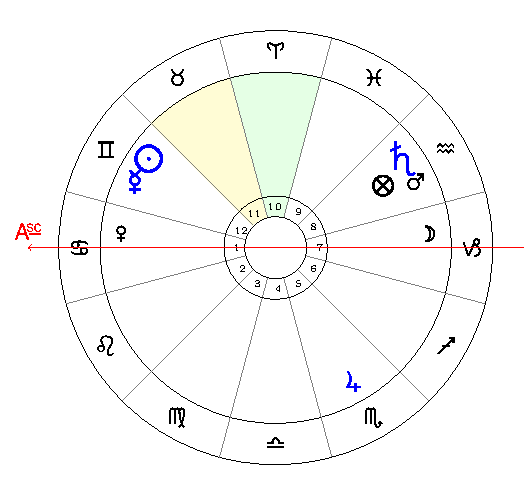
\includegraphics[width=0.68\textwidth]{charts/2_21_13}
\caption{Chart 13 [II.21.13, GH L109]}
\label{fig:chart13}
\end{wrapfigure}

This man, though born a slave, entered a noble family, attained political offices, and enjoyed honors. The rulers $<$\Saturn\xspace \Mercury$>$ of the triangle of the \Sun\xspace $<$\Gemini-\Libra-\Aquarius$>$ and of the Lot
\footnote{Lot of Fortune = Asc + (\Moon\xspace\xspace - \Sun) = 90 + (270 - 60) = 300, \Aquarius, \Saturn\xspace ruler.}
 and the exaltation were found in their own domains and in aspect with
\Jupiter. \textbf{/83P/} \Mars, \Saturn, and \Mercury\xspace were unfavorably situated and so reduced his means and made
him financially embarrassed.

\newpage
% -- Chart 13 -----------------------------------------------
\subsection*{\textit{[Chart 14 Distinguished Priest with Many Troubles and Losses]}}
\addcontentsline{toc}{subsection}{\textit{[Chart 14 [GH L62] Distinguished Priest with Many Troubles and Losses]}}

Another example: \Sun\xspace in \Aquarius, \Moon, \Jupiter\xspace in \Scorpio, \Saturn\xspace in \Cancer, \Mars, \Venus, \Mercury\xspace in \Capricorn, Ascendant in \Pisces
\footnote{\textit{Greek Horoscopes} dates the chart (L62,V) to approximately January 22, 62 AD (p.83}.

\clearpage
\begin{wrapfigure}[15]{R}{7cm}
\centering
\vspace{-20pt}
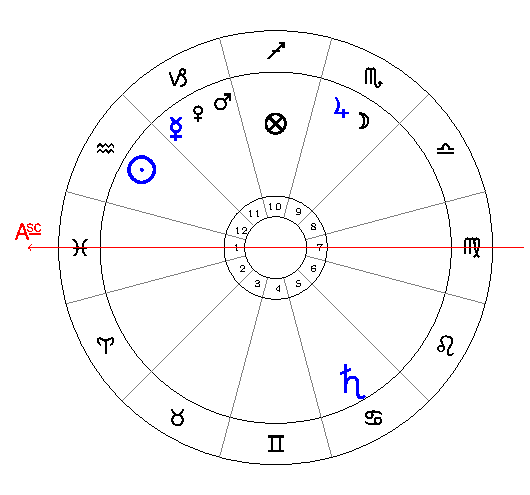
\includegraphics[width=0.68\textwidth]{charts/2_21_14}
\caption{Chart 14 [II.21.14, GH L62]}
\label{fig:chart14}
\end{wrapfigure}

This man was a eunuch, a distinguished priest of the goddess. \textbf{/87K/} The ruler $<$\Jupiter$>$ of the Lot
\footnote{Lot of Fortune = Asc + (\Moon\xspace\xspace - \Sun) = 330 + ((360+210) - 300) = 600 - 360 = 240, \Sagittarius, ruled by \Jupiter\xspace in \Scorpio.}
 happened to be in \Scorpio, $<$the IX Place of$>$ the God. The rulers of the $<$diurnal$>$ sect, \Saturn\xspace and \Mercury, were found in Good Daimon, but in opposition. Therefore he fell into a great many troubles and losses and quarrels with governors and kings.

\newpage